\documentclass{standalone}
\usepackage[utf8]{inputenc}
\usepackage{amsmath}
\usepackage{tikz}

\usetikzlibrary{decorations, decorations.pathreplacing, decorations.pathmorphing}

\begin{document}

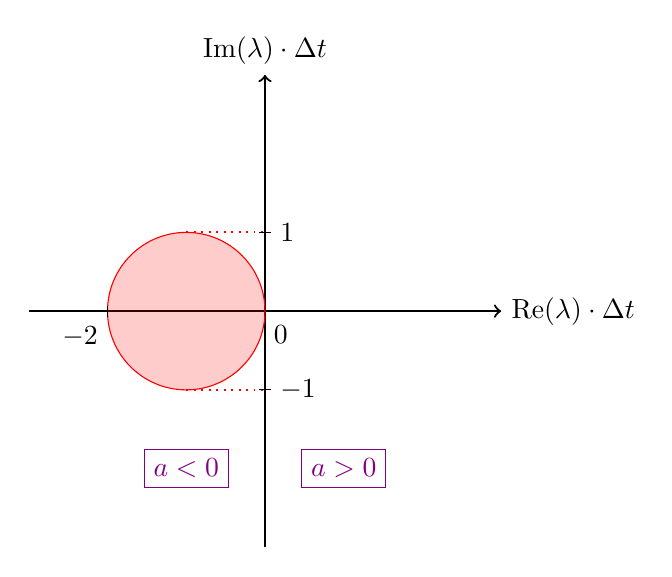
\begin{tikzpicture}
    \draw[thick,->] (-3,0) -- (3,0) node[right] {$\text{Re}(\lambda)\cdot\Delta t$};
    \draw[thick,->] (0,-3) -- (0,3) node[above] {$\text{Im}(\lambda)\cdot\Delta t$};

    \draw[fill = red,red,fill opacity=0.2] (-1,0) circle (1);

    \draw (-2 ,2pt) -- (-2,-2pt) node[anchor=north east] {$-2$};
    \node at (0.2,-0.3) {$0$};
    \draw[color=red, dotted, line width=0.7pt](-1,1)--(0,1);
    \draw[color=red, dotted, line width=0.7pt](-1,-1)--(0,-1);
    \draw (-2pt ,1) -- (2pt,1) node[right] {$1$};
    \draw (-2pt ,-1) -- (2pt,-1) node[right] {$-1$};
    \node[draw,color=violet] at (-1,-2) {$a<0$};
    \node[draw,color=violet] at (1,-2) {$a>0$};
\end{tikzpicture}

\end{document}
